Im ersten Schritt wurde die Anbindung der neuzuschaffenden Schnittstelle zur Erfassung der Daten aus dem Signatur-Tablet sowie die 
Weitergabe und Integration in den bestehenden Datenbestand der Sage Office Line durch FZP geprüft. Im zweiten Schritt wurden verschiedene
Anbieter von Signatur-Tablets geprüft. Hier hat sich die Firma Wacom schnell heraus kristallisiert, hinsichtlich der Unternehmenserfahrungen seit 1983 \cite{konzept1} sowie der guten Anbindungen des grafischen Tablets mittels des bereit gestellten SDK\footnote{\label{foot:4}Software Development Kit: Sammlung von Werkzeugen und Anwendungen, um eine Software zu erstellen, meist inklusive Dokumentation. \cite{SDK}}. Nach Abschluss der Prüfungen wurde mit der Entwicklung der Schnittstelle begonnen.
\newline
Die Entwicklung von Schnittstellen ist aufgrund des modularen Aufbaukonzepts der Sage Office Line möglich. Die Einbindung der Schnittstellen wird mit einer eigenentwickelten Methode namens DCM (DLL Common Method) realisiert. Mit dieser Methode können Anpassung an der Sage Office Line auf Basis des Microsoft .NET-Frameworks\footnote{\label{foot:5}Framework: Grundstruktur / Rahmenwerk zur Bestimmung der 
Software-Architektur. Es besteht aus mehreren Klassen, die zusammenarbeiten und wieder verwendbare Entwürfe darstellen. \cite{framework}}
vorgenommen und diese mit der verwendeten Technologie der Sage Office Line auf Basis des Microsoft COM-Frameworks verbunden werden.
\newline
Der erste Schritt ist die Einbindung der benötigten DLL\footnote{\label{foot:6}Dynamic Link Library: Dynamische Programmbibliothek für Microsoft Betriebssysteme. \cite{DLL}} in das Microsoft .NET Entwicklungsprojekt. Die DLL umfassen unteranderen die benötigten Komponenten zur Kommunikation zwischen der Schnittstelle und der Sage Office Line sowie dem Signatur-Tablet. Des Weiteren werden die DLL des Signatur-Tablets zur Erfassung und Prüfung der digitalen Signatur eingebunden. Das Entwicklungsprojekt ist in 2 Unterprojekte geteilt. Die Aufteilung in 2 Projekte wurde angesichts der Wiederverwendbarkeit von einzelnen Projektteilen gewählt.
\newline
Das in der Abbildung 5 dargestellte Klassendiagramm symbolisiert das erste Projekte. Der rot umrandete Bereich zeigt die Klassen die die Anbindung an die Sage Office Line regeln. Es existieren 2 Klassen die die Erfassungsmaske für die digitale Signatur aus der Sage Office Line heraus öffnen können. Die Erfassungsmaske kann im Standard des Verkaufsbereichs der Sage Office Line sowie im Zusatzmodul FZP Vermietung gestartet werden (siehe Abbildung 8 und 9). Der blau umrandete Bereich zeigt die Klasse der Erfassungsmaske. Die Erfassungsmaske enthält das geschaffene Steuerelement zur Erfassung der digitalen Signaur. Weiterhin regelt die Maske den Funktionsaufruf zur Speicherung der digitalen Signatur sowie das Öffnen und Schließen der Erfassungsmaske. Der grün umrandete Bereich zeigt die Klasse des Signaturbelegs. Diese Klasse dient zum Speichern, Aktualisieren und Laden von Signaturen sowie zur Prüfung, ob eine digitale Signatur bereits vorhanden ist. Weiterhin enthält der grüne Bereich eine Klasse mit Funktionen zur Prüfung der Datenbank und deren Version, zum Aktualisieren der Datenbank, zum Erstellung und Schließen einer Datenbankverbindung sowie zur Ausgabe von Hinweis- und Fehlermeldungen.
\begin{figure}[!ht]
    \centering
    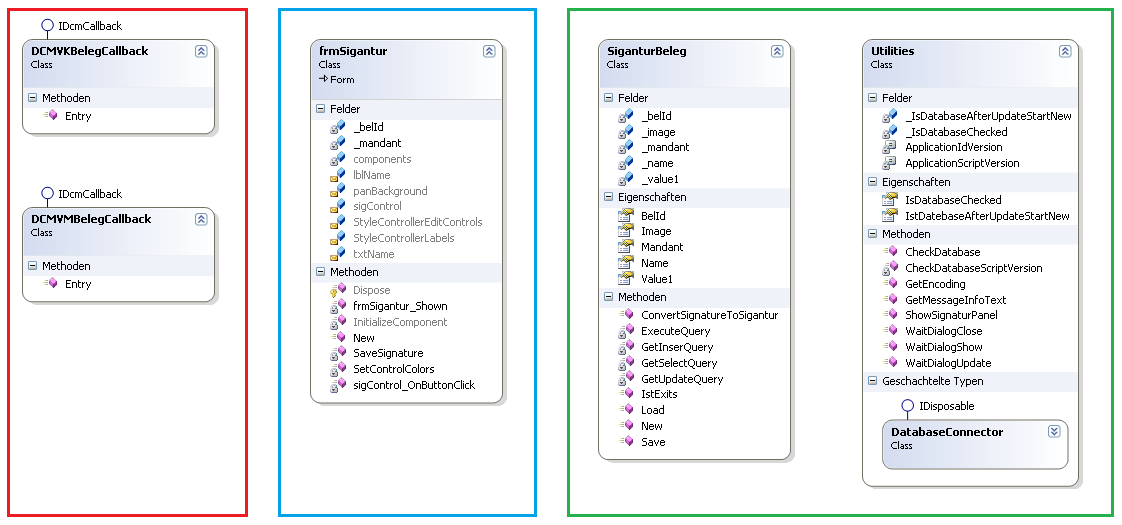
\includegraphics[height=200pt, width=450pt]{Klassendiagramm_Abf_Signatur_Edit2.png}
    \caption[Klassendiagramm Einbindung und Verarbeitung digitale Signatur]{\small{Klassendiagramm Teilprojekt Einbindung und Verarbeitung digitale Signatur}}
\end{figure}\\
Das Klassendiagramm in der Abbildung 6 symbolisert das zweite Projekt. In diesem Projekt wurde im blau umrandeten Bereich das Steuerelement zur Darstellung der digitalen Signatur auf einem Bildschirm geschaffen. Die Funktionen des Steuerelements sind die Ermittlung des verwendeten USB bzw. COM-Port des Signatur-Tablets, die Zeichnung des Erscheinungsbilds des Steuerelements, die Entfernung der Signatur vom Tablet und das Schließen des Steuerelements. Die Klassen im grün umrandeten Bereich sind für folgende Funktionen zuständig. Das Steuerelement reagiert auf die Eingaben des Signatur-Tablets und leitet diese an die Klassen zur Sammlung, Prüfung und Aufbereitung der Daten aus dem Signatur-Tablet weiter. Im nächsten Schritt der Daten an die Eingabemaske zur Darstellung weiter geleitet. Im letzten Schritt wird mit den aufbereiteten Daten die digitale Signatur erstellt und an die Klasse Signaturbeleg zur Speicherung übergeben.
\begin{figure}[!ht]
    \centering
    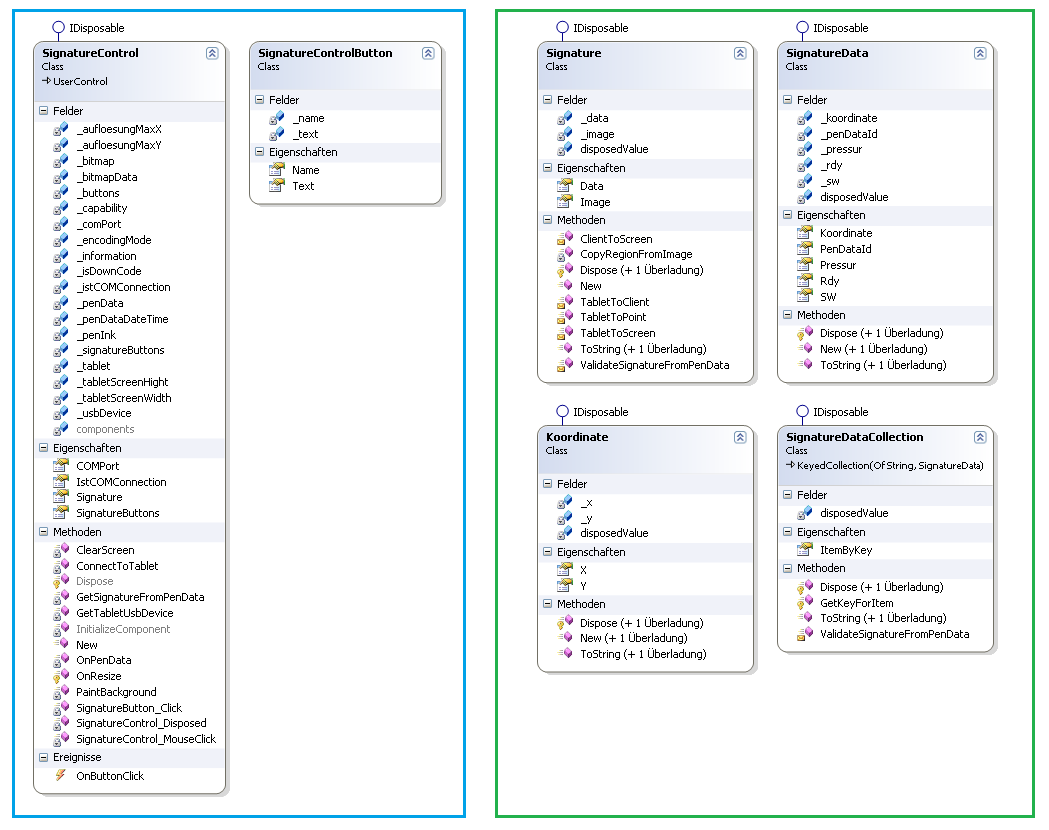
\includegraphics[height=350pt, width=450pt]{Klassendiagramm_FZP_Wacom_Edit1.png}
    \caption[Klassendiagramm Erstellung Steuerelement und Aufbereitung Daten]{\small{Klassendiagramm Teilprojekt Erstellung Steuerelement und Aufbereitung Daten}}
\end{figure}\\
Die Speicherung der Daten der digitalen Signatur erfolgt in einer MS-SQL Datenbank. Die Sage Office Line benutzt ebenso MS-SQL Datenbanken und somit ist die Einbindung der neugeschaffenen Datenbanktabellen in das bestehende Datenbankschema problemlose zu bewerkstelligen. Ein weiterer Grund für die Nutzung von MS-SQL ist die hohe Sicherheit, die Wiederverwendbarkeit sowie eine geringe Wahrscheinlichkeit von Datenverlust aufgrund regelmäßiger Datenbanksicherungen.